% \begin{figure}
% \centering
% 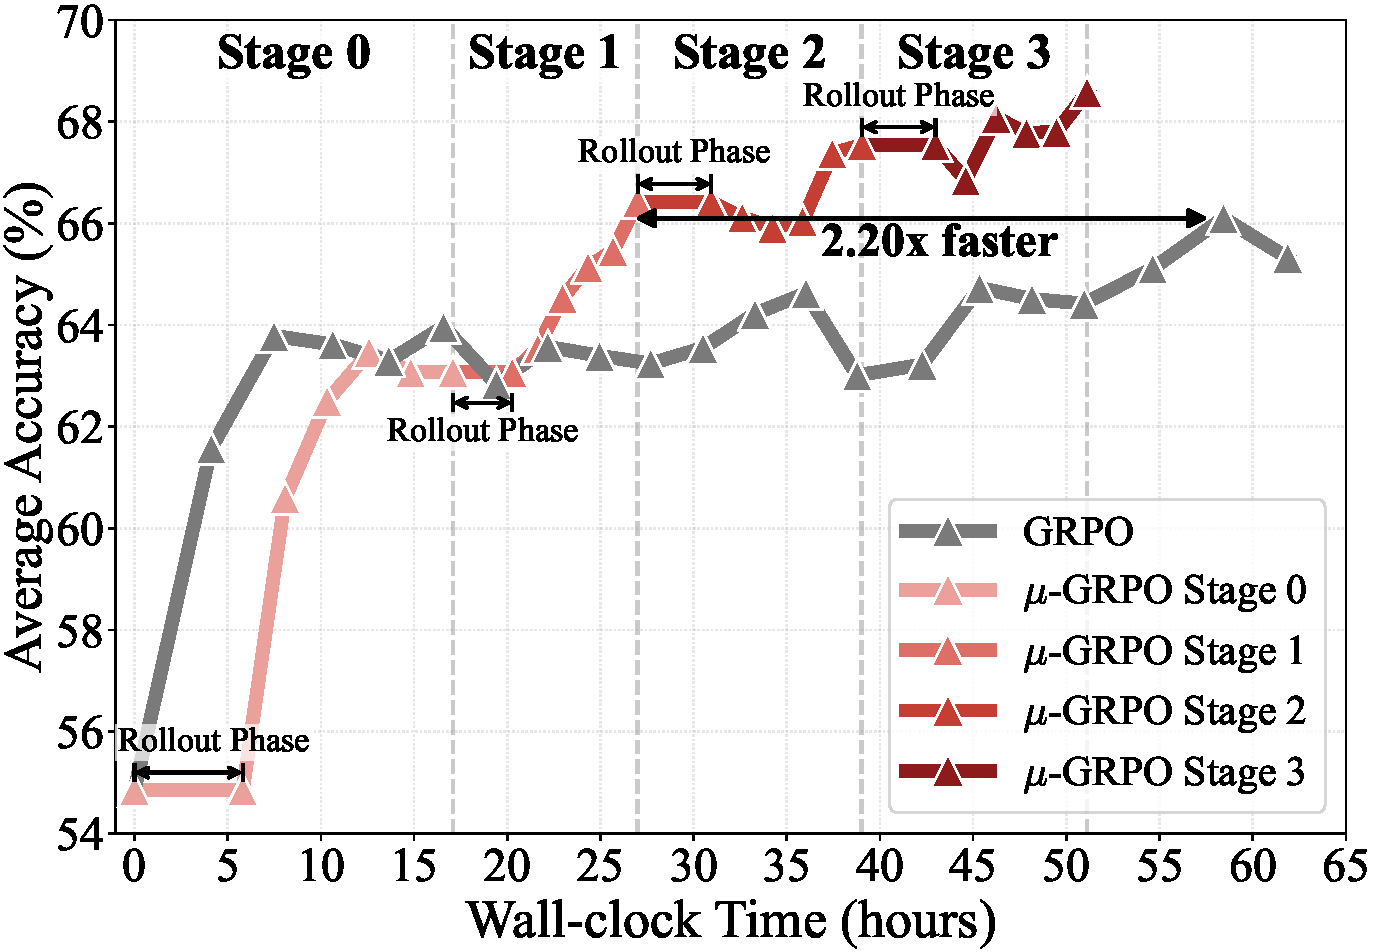
\includegraphics[width=0.47\textwidth]{figures/teaser.pdf}
% \caption{Wall-clock efficiency comparison between on-policy GRPO ($\mu\!=\!4$) and high-staleness $\mu$-GRPO ($\mu\!=\!1024$) over 4096 model updates, evaluated on DeepSeek-7B \citep{shao2024deepseekmathpushinglimitsmathematical}.
% Curves show average accuracy (\%) across five evaluation benchmarks as a function of wall-clock time (hours).
% Stage durations are non-uniform, reflecting changes in the model’s mean response length during training, which affect rollout generation and per-step computation costs and thus result in varying wall-clock times.}
%     \label{fig:teaser}
% \end{figure}


\begin{wrapfigure}{r}{0.6\linewidth}
% \vspace{-pt}
\centering
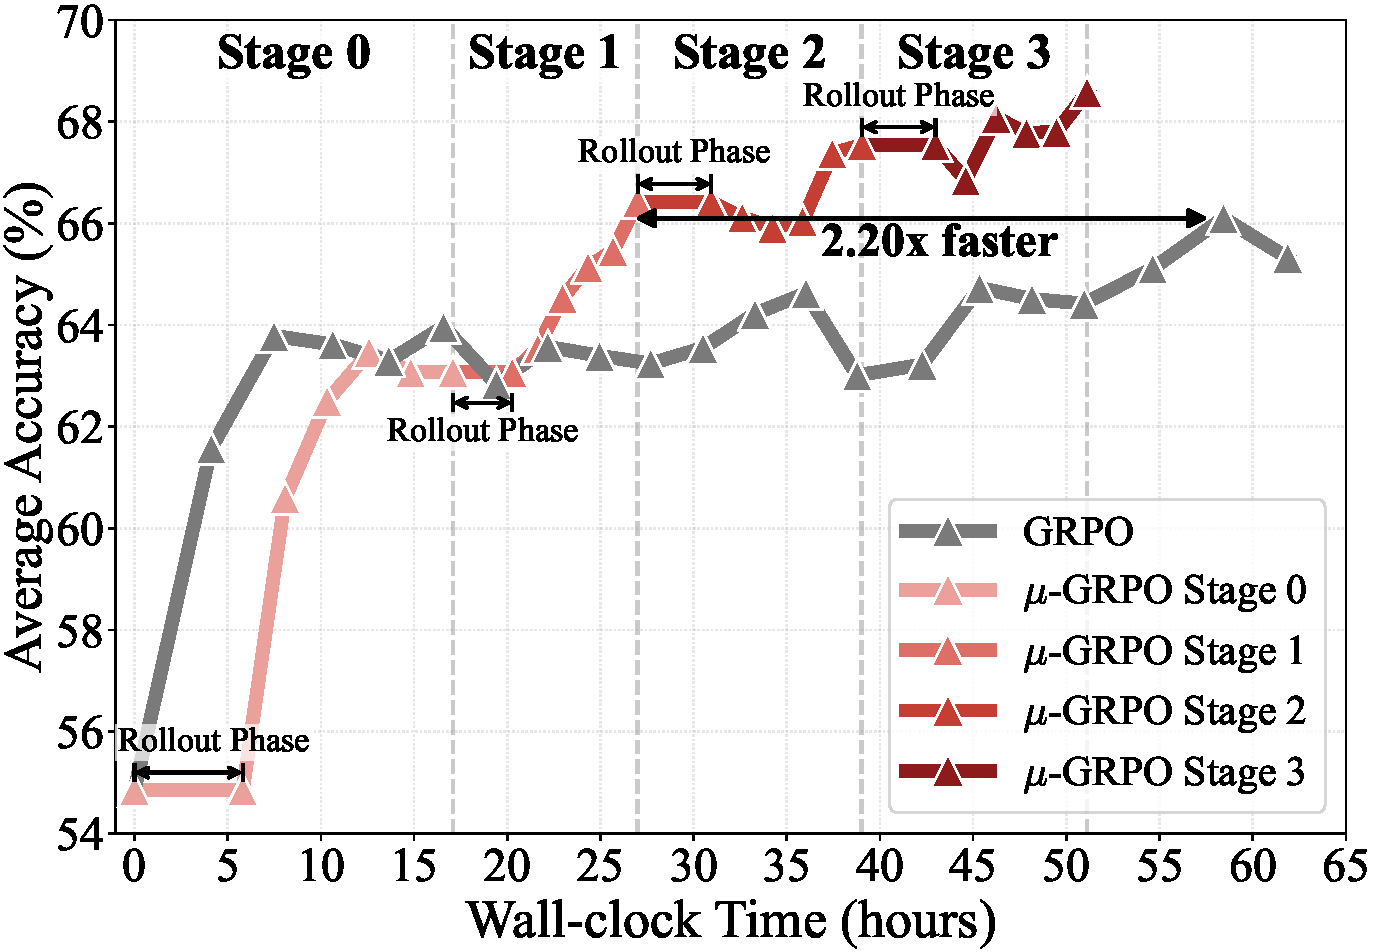
\includegraphics[width=\linewidth]{figures/teaser.pdf}
\caption{
\textbf{Comparing GRPO and \boldmath \ourmethod.}
Average accuracy across five math benchmarks over
wall-clock time. \ourmethod{} uses four large rollout--optimization stages, inducing high rollout
staleness while reducing rollout--training switching overhead. It reaches GRPO's
performance with a 2.2$\times$ wall-clock speedup on DeepSeek-7B~\citep{shao2024deepseekmathpushinglimitsmathematical}.
Both methods are trained for 4096 updates.
}
\label{fig:teaser}
\vspace{-14pt}
\end{wrapfigure}